\chapter{Теория графов}
\section{Основные определения}
Пусть $M$ и $N$ - два конечных множества. Будем называть пару множеств $\langle M, N \rangle$ \textbf{ориентированным графом}.
При этом элементы множества $M$ называются \textbf{вершинами} графа, элементы множества $N$ - \textbf{дугами} графа. 
Граф, у которого направления соединения не определены, называется \textbf{неориентированным графом}. В них
соединения называются \textbf{ребром}, а вершина - \textbf{узлом}.

\begin{figure*}[!h]
    \centering
    \begin{minipage}[t]{4cm}
        \centering
        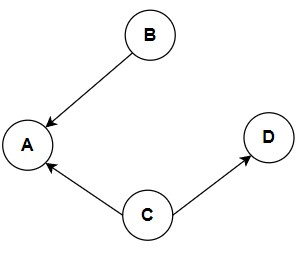
\includegraphics{graph_or.jpg}
        \caption{Ориентированный граф}
    \end{minipage}
    \hspace{3cm}
    \begin{minipage}[t]{4cm}
        \centering
        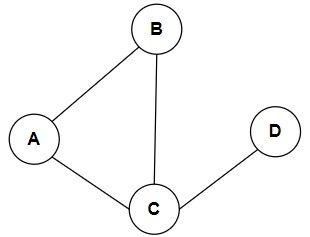
\includegraphics{graph_nor.jpg}
        \caption{Неориентированный граф}
    \end{minipage}
\end{figure*}

\textbf{Висячей вершиной} называется вершина, которая соединена только с одной соседней вершиной.

\textbf{Степенью вершины} называется количество ребер, соединенных с этой вершиной.
Если степень вершины равна 0, то такая вершина называется \textbf{изолированной}.
Степень вершины может быть \textbf{входящей} и \textbf{исходящей}. Входящая степень вершины $v$
это количество ребер вида $\langle i, v \rangle$, то есть количество ребер которые входят в $v$.
Исходящая степень вершины $v$ это количество ребер вида $\langle v, i \rangle$, то есть количество ребер
которые входят из $v$.

\begin{thm}
    В любом графе всегда найдутся хотя бы две вершины с одинаковой степенью.
\end{thm}

Дуга, у которой начало и конец совпадают, называется \textbf{петлей}.

Граф $\langle M', N'\rangle$ называется \textbf{простым путем}, если
\begin{enumerate}
    \item число его дуг $k$ на единицу меньше числа вершин
    \item можно так пронумеровать $M'$ числами от 0 до $k$ и $N'$ числами от 1 до $k$,
    что для любой дуги $u \in N'$
\end{enumerate}

Пусть $num$ - это получение номера дуги или вершины, а $beg(u)$ и $end(u)$ начало и конец дуги 
$u$ соответственно. Тогда для любой дуги $u$ в графе верно выражение:
\begin{equation}
    \label{simple_path}
    num(u) = num(end(u)) = num(beg(u)) + 1
\end{equation}
Различие между \textbf{путем} и \textbf{простым путем} заключается в том, что во втором случае
недопустимы повторы вершин и дуг в пути.
\begin{figure}[h]
    \centering 
    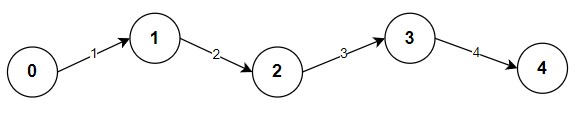
\includegraphics{simple_path.jpg}
    \caption{Простой путь}
\end{figure}

\begin{thm}
    Простым графом называется граф, который не имеет петель и не содержит более чем одно ребро между вершинами.
\end{thm}
Граф $\langle M', N'\rangle$ называется \textbf{цепью}, если:
\begin{enumerate}
    \item число его дуг $k$ на единицу меньше числа вершин
    \item можно так пронумеровать $M'$ числами от 0 до $k$ и $N'$ числами от 1 до $k$,
    что для любой дуги $u \in N'$
\end{enumerate}
То есть, он включает либо условие простого пути \ref{simple_path}, либо
\begin{equation}
    \label{chain}
    num(u) = num(end(u)) + 1 = num(beg(u))
\end{equation}
Дуги, для которых выполняется \ref{simple_path}, принято называть \textbf{положительно ориентированными},
а те, для которых выполняется \ref{chain} \textbf{отрицательно ориентированными}.

\begin{figure}[h]
    \centering 
    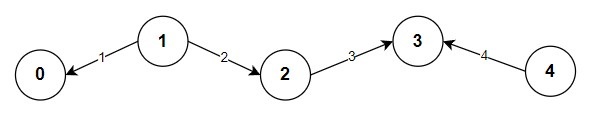
\includegraphics{chain.jpg}
    \caption{Цепь}
\end{figure}

Граф $\langle M', N'\rangle$ называется \textbf{контуром}, если
\begin{enumerate}
    \item число дуг $k$ равно числу вершин
    \item можно так пронумеровать $M'$ и $N'$ числами от 1 до k, что для любой
    дуги $u \in N'$
\end{enumerate}
\begin{equation}
    num(u) \stackrel{\text{mod k}}{=} num(end(u)) \stackrel{\text{mod k}}{=} num(beg(u)) + 1
\end{equation}
Иными словами, контур - это простой путь, где начало и конец совпадают.

\begin{figure}[h]
    \centering 
    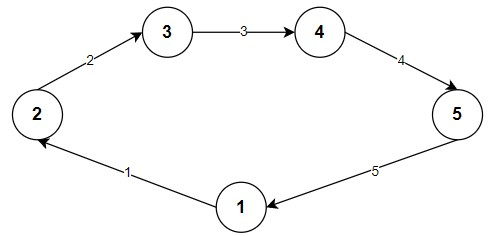
\includegraphics{loop.jpg}
    \caption{Контур}
\end{figure}

\vspace{3mm}

Граф $\langle M', N'\rangle$ называется \textbf{циклом}, если
\begin{enumerate}
    \item число дуг $k$ равно числу вершин
    \item можно так пронумеровать $M'$ и $N'$ числами от 1 до $k$, что для любой дуги $u \in N'$
\end{enumerate}
\begin{equation}
    num(u) \stackrel{\text{mod k}}{=} num(end(u)) \stackrel{\text{mod k}}{=} num(beg(u)) + 1
\end{equation}
либо
\begin{equation}
    num(u) \stackrel{\text{mod k}}{=} num(end(u)) + 1 \stackrel{\text{mod k}}{=} num(beg(u))
\end{equation}
Цикл - это цепь, в которой начало и конец совпадают.
\begin{figure}[h]
    \centering 
    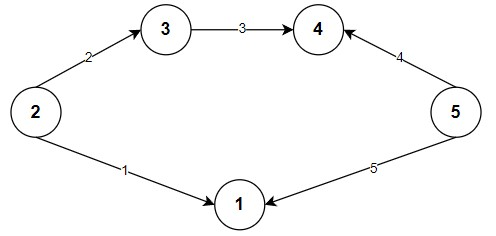
\includegraphics{cycle.jpg}
    \caption{Цикл}
\end{figure}

\section{Связность. Компоненты связности и сильной связности}
Граф $\langle M, N\rangle$ называется \textbf{связным}, если любые две различные его
вершины можно соединить цепью. Любой граф может быть однозначно разделен на максимальные
связные подграфы, которые называют его \textbf{компонентами связаности}.
c

Граф $\langle M, N\rangle$ называется \textbf{сильно связным}, если любые две различные
вершины A и B можно соединить путем с началом в A и концом в B. В любом графе можно однозначно
выделить максимальные сильно связные подграфы, которые называются его \textbf{компонентами сильной связности}.
\begin{thm}
    Граф компонент сильной связности не имеет контуров.
\end{thm}

\section{Матричные представления графов}
Прежде чем приступить к понятию "дерево" , изучим различные способы представления графов.
Наиболее известные формы это \textbf{матрица инцидентности} и \textbf{матрица смежности}.
Для начала рассмотрим более простой вариант - матрицу смевжности.

\vspace{3mm}

\textbf{Матрицей смежности} графа $\langle M, N\rangle$ называется такая квадратная матрица $M \times M$
(то есть индексами строк и столбцов являются вершины графа), 
в которой значением пересечения $i$-ой строки и $j$-го столбца является число дуг с началом в $i$ и концом $j$.

\begin{figure}[!h]
    \centering 
    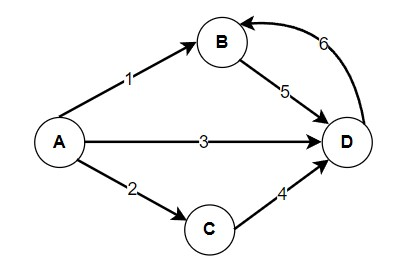
\includegraphics{graph_1.jpg}
    \caption{Граф}
    \label{graph_for_matrix}
\end{figure}

\begin{figure*}[!h]
    \centering
    \begin{minipage}[t]{4cm}
        \centering
        \begin{tabular}[c]{ | l | l | l | l | l | l | l | l |}
            \hline
              & 1  & 2  & 3  & 4  & 5  & 6  \\ \hline
            A & 1  & 1  & 1  & 0  & 0  & 0  \\ \hline
            B & -1 & 0  & 0  & 0  & 1  & -1 \\ \hline
            C & 0  & -1 & 0  & 1  & 0  & 0  \\ \hline
            D & 0  & 0  & -1 & -1 & -1 & 1  \\
            \hline
        \end{tabular}
    \end{minipage}
    \hspace{3cm}
    \begin{minipage}[t]{4cm}\
        \centering
        \begin{tabular}[c]{ | l | l | l | l | l |}
            \hline
              & A & B & C & D \\ \hline
            A & 0 & 1 & 1 & 1 \\ \hline
            B & 0 & 0 & 0 & 1 \\ \hline
            C & 0 & 0 & 0 & 1 \\ \hline
            D & 0 & 1 & 0 & 0 \\
            \hline
        \end{tabular}
    \end{minipage}
    \caption{Способы матричного представления графа \ref{graph_for_matrix}: матрица инцидентности
    и матрица смежности соответственно}
\end{figure*}

\hspace{3mm}

\textbf{Матрицей инцидентности} графа $\langle M, N\rangle$ называется такая матрица $M \times N$, 
где индексами строк являются вершины, а индексами столбцов дуги. Элемент на пересечении $i$-ой строки и $j$-ого
столбца равен 1, если является началом в вершине под $i$-ым индексом и принадлежит дуге под $j$-ым индексом. Если же данная
дуга имеет конец в этой вершине, то ставится -1.

\section{Деревья}
Чтобы ввести термин "дерево", нам нужно изучить следующую теорму:
\begin{thm}
    В связном графе $\langle M, N \rangle$ найдется частичный граф связный граф
    $\langle M, N' \rangle$, в котором количество вершин больше количества дуг на единицу. Пусть $|N'| = k$, 
    тогда если пронумеровать вершины из M числами от 0 до k, а дуги из N' числами от 1 до k
    таким образом, что для любой дуги $u \in N'$ выполняется соотношение
    \begin{equation}
        num(u) = max\{num(beg(u)), num(end(u))\}
    \end{equation}
\end{thm}
\begin{sle}
    Если $|N| < |M| - 1$, граф не может быть связан.
\end{sle}
\begin{sle}
    Если $|N| > |M| - 1$, граф содержит циклы.
\end{sle}

Связный граф без циклов, в котором число дуг на 1 меньше числа вершин, называется
\textbf{деревом}. Такие деревья могут не иметь корня, в отличие от тех деревьев,
которые мы обычно представляем. Если подобное дерево имеет корень, то оно называется 
\textbf{ориентированным деревом}.

\begin{thm}
    Для того, чтобы простой неориентированный граф с n вершинами был деревом необходимо 
    и достаточно, чтобы он был связен  и в нем было n-1 ребро.
\end{thm}
Дерево, являющееся частичным графом связного графа, называется его \textbf{остовным деревом} (spanning tree).

Теперь можно присутпить к изучению алгоритма нахождения остовного дерева методом вычеркивания.

\hspace{5mm}
\newpage

\section{Алгоритмы нахождения остовного дерева}
\textbf{Алгоритм ближайшего соседа}
\begin{enumerate}
    \item В весовой матрице выбираем произвольную вершину.
    \item Ищем в этой весовой вершине минимальную дугу в другую вершину.
    \item Ищем среди этих вершин снова минимальную дугу уже в новую вершину.
    \item Продолжаем до тех пор, пока не пометим все вершины.
\end{enumerate}
Приведем пример. Пусть есть следующая весовая матрица:

\begin{table}[h]
    \centering
    \begin{tabular}[c]{ | l | l | l | l | l | l | l | }
        \hline
          & A & B & C & D & E & F \\ \hline
        A & 0 & 0 & $\infty$ & 4 & 6 & $\infty$ \\ \hline
        B & 5 & 0 & $\infty$ & 7 & 5 & 4\\ \hline
        C & $\infty$ & $\infty$ & 0 & 5 & 6 & 4 \\ \hline
        D & 4 & 7 & 5 & 0 & 8 & 3\\ \hline
        E & 6 & 5 & 6 & 8 & 0 & $\infty$\\ \hline
        E & $\infty$ & 4 & 4 & 3 & $\infty$ & 0 \\
        \hline
    \end{tabular}
    \caption{Весовая матрица}
\end{table}

\begin{figure}[!h]
    \centering 
    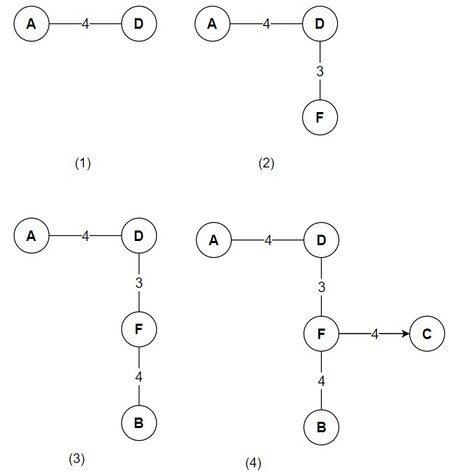
\includegraphics{kn.jpg}
    \caption{Алгоритм ближайшего соседа}
    \label{graph_kn}
\end{figure}

На рисунке \ref{graph_kn} изображен алгоритм построения остовного дерева для весовой матрицы выше. 
Пусть произвольная вершина будет A. Минимальное ребро идет в вершину D. 
Далее выбираем среди этих двух вершин минимальное ребро, и это D -> F. По такому же
алгоритму достраиваем остовное дерево.

\hspace{5mm}
\newpage
\textbf{Жадный алгоритм}

Этот алгоритм основан по большей части на том, что каждый раз мы выбираем минимальное ребро
на каждом этапе, а далее объединяем полученные ребра в остовное дерево. Для той же весовой матрицы покажем:
На рисунке \ref{greedy_alg} изображено построение остовного дерева с помощью жадного алгоритма.

\begin{figure}[!h]
    \centering 
    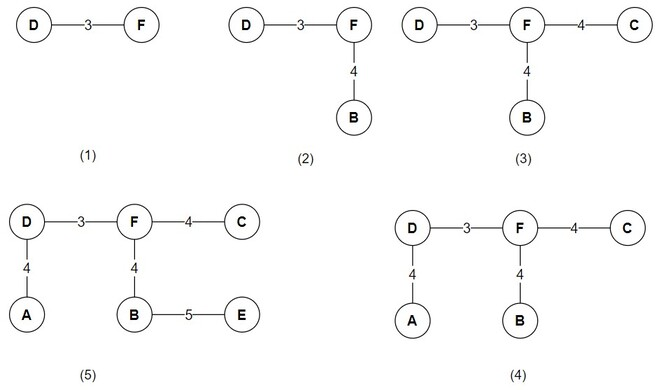
\includegraphics{greedy_alg.jpg}
    \caption{Жадный алгоритм}
    \label{greedy_alg}
\end{figure}

Самое минимальное ребро равно 3 с вершинами D и F. Далее мы имеем 3 равнозначеных ребра равных 4:
F и B, F и C, D и A. Строми последовательно их. Не хватает последнего ребра E. Можно заметить, что самое минимальное
ребро с этой вершиной из B. Остовное дерево построено.

\hspace{5mm}
\newpage
\textbf{Алгоритм вычеркивания}

\begin{enumerate}
    \item В матрице инцидентности $N \times N-1$ проверяем наличие нулевых строк. 
    Если есть, то имеем неостовное дерево.
    \item Если нет, то проверяем наличие строк с одной единицей
    и вычеркиваем строку и столбец, проходящие через эту единицу
    \item Повторяем пункт 1 и 2 до тех пор, пока не придем к выводу, что это неостовное дерево или
    если все столбцы вычеркнуты, то рассмотренные ребра образуют остовное дерево
\end{enumerate}

Рассмотрим пример. Имеем следующую матрицу инцидентности:
\begin{table}[!h]
    \centering
    \begin{tabular}[c]{ | l | l | l | l | l | l | l | l | l | l | }
        \hline
        1 & 2 & 3 & 4 & 5 & 6 & 7 & 8 & 9 & 10 \\ \hline
        1 & 0 & 0 & 1 & 0 & 1 & 0 & 0 & 0 & 0 \\ \hline
        0 & 1 & 0 & 0 & 0 & 0 & 0 & 0 & 1 & 1 \\ \hline
        1 & 1 & 1 & 0 & 0 & 0 & 0 & 0 & 0 & 0 \\ \hline
        0 & 0 & 0 & 0 & 0 & 1 & 1 & 1 & 0 & 0 \\ \hline
        0 & 0 & 1 & 0 & 0 & 1 & 1 & 0 & 0 & 0 \\ \hline
        0 & 0 & 0 & 1 & 1 & 0 & 0 & 0 & 0 & 0 \\ 
        \hline
    \end{tabular}
    \caption{Матрица инцидентности}
\end{table}
\newpage
Теперь проверим, являются ли ребра 1, 2, 5, 7 и 8 остовным деревом:
\begin{figure}[!h]
    \centering 
    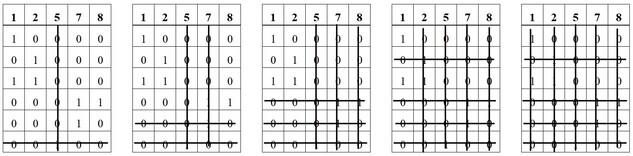
\includegraphics{matrix1.jpg}
    \caption{Алгоритм вычеркивания}
\end{figure}

Так как в процессе у нас не возникло нулевых строк и в итоге все строки и столбцы 
были зачеркнуты, данные ребра образуют остовное дерево.
Например, ребра 1, 2, 4, 5 и 8 не будут образовывать остовное дерево, так как 5
строчка будет состоять только из нулей.

\section{Задача о кратчайшем пути}
Для того чтобы найти кратчайший путь от одной вершины до других, используется алгоритм Дейкстры.
Алгоритм работает только для графов без рёбер отрицательного веса.

Алгоритм заключается в том, что каждой вершине соотвествует минимальное известное расстояние от
этой вершины до \textbf{a}. Метка вершины \textbf{a}, от которой ищутся кратчайшие расстояния до других, изначально равна 0, метки
остальных вершин равны бесконечности. Алгоритм работает пошагово - на каждом шаге он посещает одну вершину
и пытается уменьшать метки: из еще непосещенных вершин выбирается та, которая имеет
минимальную метку. Для каждого непосещенного соседа вершины, рассмотрим новую длину пути,
равную сумме значений текущей метки и длины ребра, соединяющего ее с этим соседом.
Если все вершины посещены, то работа алгоритма прекращается. Рассмотрим теперь пример:

\hspace{3mm}

Пусть требуется найти кратчайшие расстояния от 1-й вершины до всех остальных. 

\begin{figure}[!h]
    \centering
    \begin{tabular}{cc}
        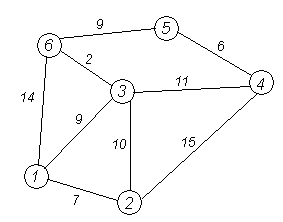
\includegraphics[scale=0.6]{dijkstra_1.png} & 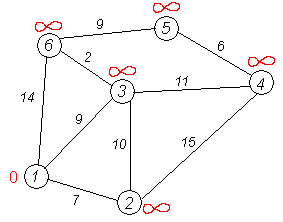
\includegraphics[scale=0.6]{dijkstra_2.png}
    \end{tabular}
\end{figure}

Кружками обозначены вершины, линиями — пути между ними (рёбра графа).
В кружках обозначены номера вершин, над рёбрами обозначен их вес — длина пути.
Рядом с каждой вершиной красным обозначена метка — длина кратчайшего пути в эту вершину из вершины 1. 

Минимальную метку имеет вершина 1. Её соседями являются вершины 2, 3 и 6.

Первый по очереди сосед вершины 1 — вершина 2, потому что длина пути до неё минимальна.
Длина пути в неё через вершину 1 равна сумме значения метки вершины 1 и длины ребра, идущего из 1-й в 2-ю, то есть 0 + 7 = 7.
Это меньше текущей метки вершины 2, бесконечности, поэтому новая метка 2-й вершины равна 7.
Аналогичную операцию проделываем с двумя другими соседями 1-й вершины — 3-й и 6-й.

\begin{figure}[!h]
    \centering 
    \begin{tabular}{cc}
        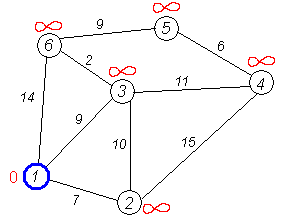
\includegraphics[scale=0.6]{dijkstra_3.png} & 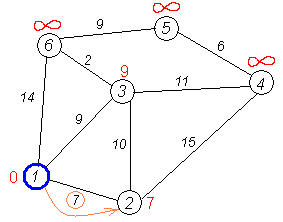
\includegraphics[scale=0.6]{dijkstra_4.png} \\
        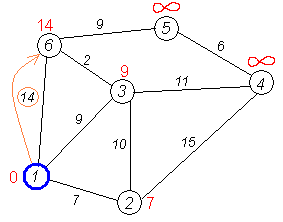
\includegraphics[scale=0.6]{dijkstra_5.png} & 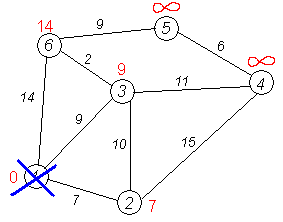
\includegraphics[scale=0.6]{dijkstra_6.png}
    \end{tabular}
\end{figure}
\newpage
Все соседи вершины 1 проверены.
Текущее минимальное расстояние до вершины 1 считается окончательным и пересмотру не подлежит.
Вычеркнем её из графа, чтобы отметить, что эта вершина посещена. 

Снова находим «ближайшую» из непосещённых вершин. Это вершина 2 с меткой 7. 

\begin{figure}[!h]
    \centering 
    \begin{tabular}{cc}
        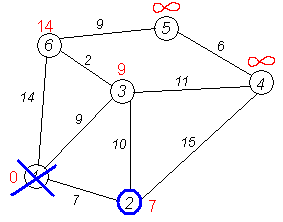
\includegraphics[scale=0.6]{dijkstra_7.png} & 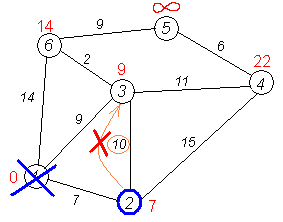
\includegraphics[scale=0.6]{dijkstra_8.png} \\
        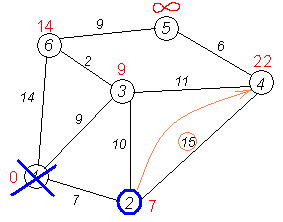
\includegraphics[scale=0.6]{dijkstra_9.png} & 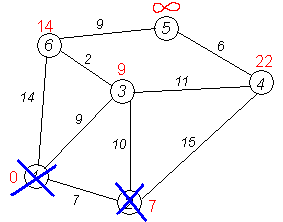
\includegraphics[scale=0.6]{dijkstra_10.png}
    \end{tabular}
\end{figure}

Снова пытаемся уменьшить метки соседей выбранной вершины, пытаясь пройти в них через 2-ю вершину. Соседями вершины 2 являются вершины 1, 3 и 4.
Первый (по порядку) сосед вершины 2 — вершина 1. Но она уже посещена, поэтому с 1-й вершиной ничего не делаем.
Следующий сосед — вершина 3, так как имеет минимальную метку.
Если идти в неё через 2, то длина такого пути будет равна 17 (7 + 10 = 17). Но текущая метка третьей вершины равна 9, а это меньше 17, поэтому метка не меняется. 
Ещё один сосед вершины 2 — вершина 4.
Если идти в неё через 2-ю, то длина такого пути будет равна сумме кратчайшего расстояния до 2-й вершины и расстояния между вершинами 2 и 4, то есть 22 (7 + 15 = 22).
Поскольку 22 < $\infty$ , устанавливаем метку вершины 4 равной 22.
Все соседи вершины 2 просмотрены, замораживаем расстояние до неё и помечаем её как посещённую. 

Проводим аналогичные шаги с другими вершинами и получаем в результате:

\begin{figure}[!h]
    \centering 
    \begin{tabular}{cc}
        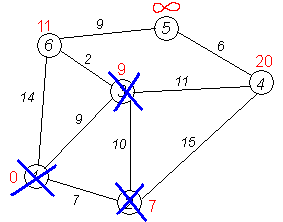
\includegraphics[scale=0.5]{dijkstra_11.png} & 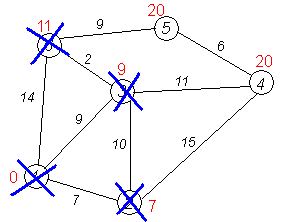
\includegraphics[scale=0.5]{dijkstra_12.png} \\
        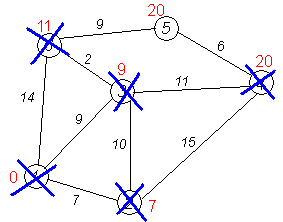
\includegraphics[scale=0.5]{dijkstra_13.png} & 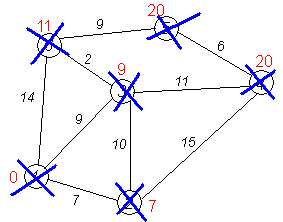
\includegraphics[scale=0.5]{dijkstra_14.png}
    \end{tabular}
\end{figure}

Алгоритм заканчивает работу, когда все вершины посещены.
Результат работы алгоритма виден на последнем рисунке: кратчайший путь от вершины 1 до 2-й составляет 7, до 3-й — 9, до 4-й — 20, до 5-й — 20, до 6-й — 11.
Если в какой-то момент все непосещённые вершины помечены бесконечностью, то это значит, что до этих вершин нельзя добраться (то есть граф несвязный). Тогда алгоритм может быть завершён досрочно. 